\documentclass[main.tex]{subfiles}
\begin{document}
\begin{bmcsex}{Effect of embedded length on the pull-out response with softening bond
    }{e44_po_softening_length_dependence}
\noindent This study shows the application of the bond-slip law
    with softening bond behavior for the simulation of a pull-out test. 
     \\
\begin{center}
            
{\scriptsize 
\begin{longtable}{lrp{4cm}}\toprule
\textbf{\textsf{Model parameter}} 
& 
\textbf{\textsf{Symbol = Value [Unit]}} 
&
\textbf{\textsf{Description}}  \\\midrule \midrule
\texttt{k\_max} & None = 1000 [None] & {\footnotesize None}  \\
            \texttt{fixed\_boundary} & None = non-loaded end (matrix) [None] & {\footnotesize which side of the specimen is fixed}  \\
            \texttt{u\_f0\_max} & $u_{\mathrm{f},0,{\max}}$ = 3.0 [mm] & {\footnotesize maximum displacement of the pulled reinforcement}  \\
            \texttt{mats\_eval\_type} & None = damage-plasticity [None] & {\footnotesize None}  \\
            \texttt{tolerance} & None = 0.0001 [None] & {\footnotesize None}  \\
            \texttt{n\_e\_x} & $n_\mathrm{E}$ = 100 [-] & {\footnotesize number of finite elements along the embedded length}  \\
            \midrule
\multicolumn{3}{l}{\textbf{\textsf{Geometry: geometry}}}\\

\texttt{geometry.L\_x} & $L$ = 100.0 [$\mathrm{mm}$] & {\footnotesize embedded length}  \\
            \midrule
\multicolumn{3}{l}{\textbf{\textsf{CrossSection: cross\_section}}}\\

\texttt{cross\_section.A\_f} & $A_\mathrm{f}$ = 16.67 [$\mathrm{mm}^2$] & {\footnotesize reinforcement area}  \\
            \texttt{cross\_section.A\_m} & $A_\mathrm{m}$ = 1540.0 [$\mathrm{mm}^2$] & {\footnotesize matrix area}  \\
            \texttt{cross\_section.P\_b} & $P_\mathrm{b}$ = 1.0 [$\mathrm{mm}$] & {\footnotesize perimeter of the bond interface}  \\
            \midrule
\multicolumn{3}{l}{\textbf{\textsf{MATSBondSlipDP: mats\_eval}}}\\

\texttt{mats\_eval.s\_0} & None = 0.00348837209302 [None] & {\footnotesize Elastic strain/displacement limit}  \\
            \texttt{mats\_eval.E\_m} & None = 30000.0 [None] & {\footnotesize None}  \\
            \texttt{mats\_eval.omega\_fn\_type} & None = li [None] & {\footnotesize None}  \\
            \texttt{mats\_eval.E\_b} & $E_\mathrm{b}$ = 12900.0 [MPa] & {\footnotesize Bond stiffness}  \\
            \texttt{mats\_eval.E\_f} & None = 200000.0 [None] & {\footnotesize None}  \\
            \texttt{mats\_eval.tau\_bar} & $\bar{\tau}$ = 45.0 [None] & {\footnotesize Reversibility limit}  \\
            \texttt{mats\_eval.uncoupled\_dp} & None = False [None] & {\footnotesize None}  \\
            \texttt{mats\_eval.K} & $K$ = 100000.0 [None] & {\footnotesize Isotropic hardening modulus}  \\
            \texttt{mats\_eval.gamma} & $\gamma$ = 0.0 [None] & {\footnotesize Kinematic hardening modulus}  \\
            \midrule
\multicolumn{3}{l}{\textbf{\textsf{LiDamageFn: omega\_fn}}}\\

\texttt{mats\_eval.omega\_fn.s\_0} & $s_0$ = 0.00348837209302 [None] & {\footnotesize elastic strain limit}  \\
            \texttt{mats\_eval.omega\_fn.alpha\_2} & $\alpha_2$ = 50.0 [None] & {\footnotesize parameter controls the damage function}  \\
            \texttt{mats\_eval.omega\_fn.alpha\_1} & $\alpha_1$ = 1.0 [None] & {\footnotesize parameter controls the damage function}  \\
            
\multicolumn{3}{r}{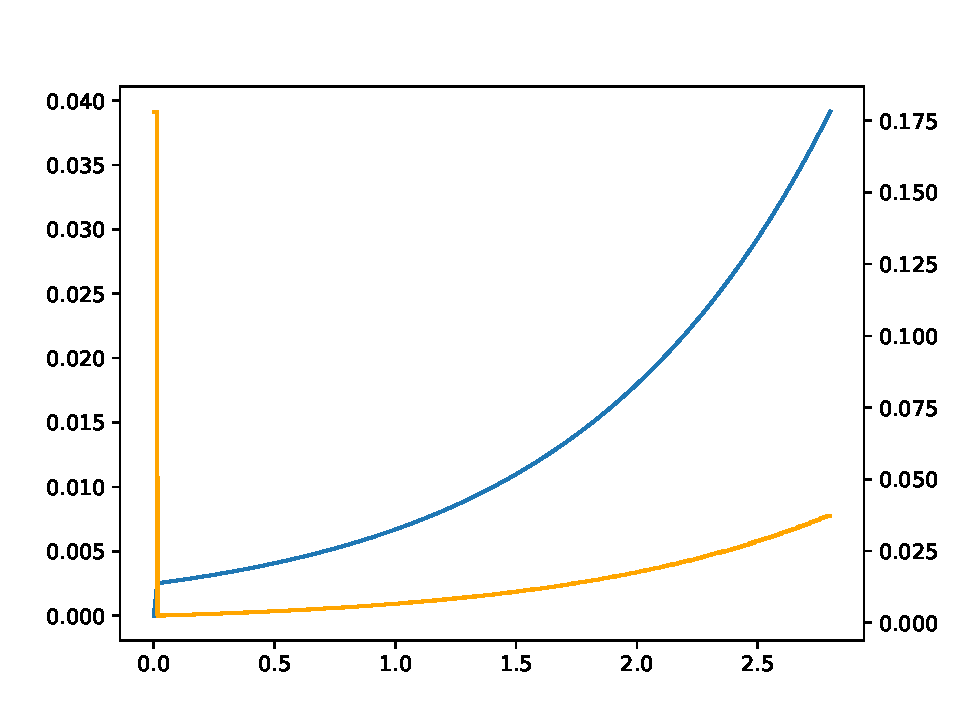
\includegraphics[width=5cm]{examples/e44_po_softening_length_dependence/fig_Li_damage_function.pdf}}\\
\bottomrule 
\end{longtable}
}

    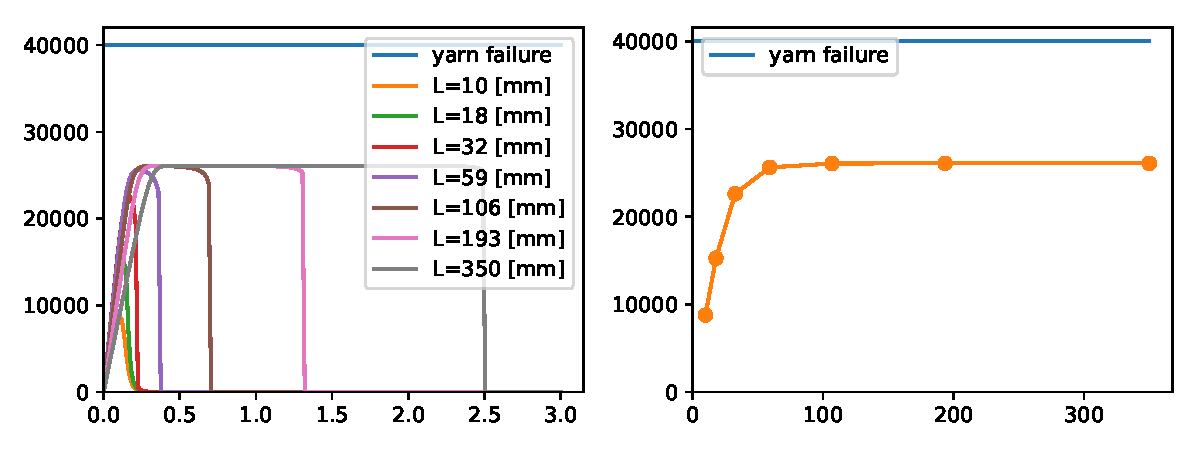
\includegraphics[width=0.95\textwidth]{examples/e44_po_softening_length_dependence/fig_length_dependence.pdf}
    \end{center}
            \end{bmcsex}
\end{document}
    